% 天文学常识

\subsection{太阳系模型}

\begin{figure}[ht]
\centering
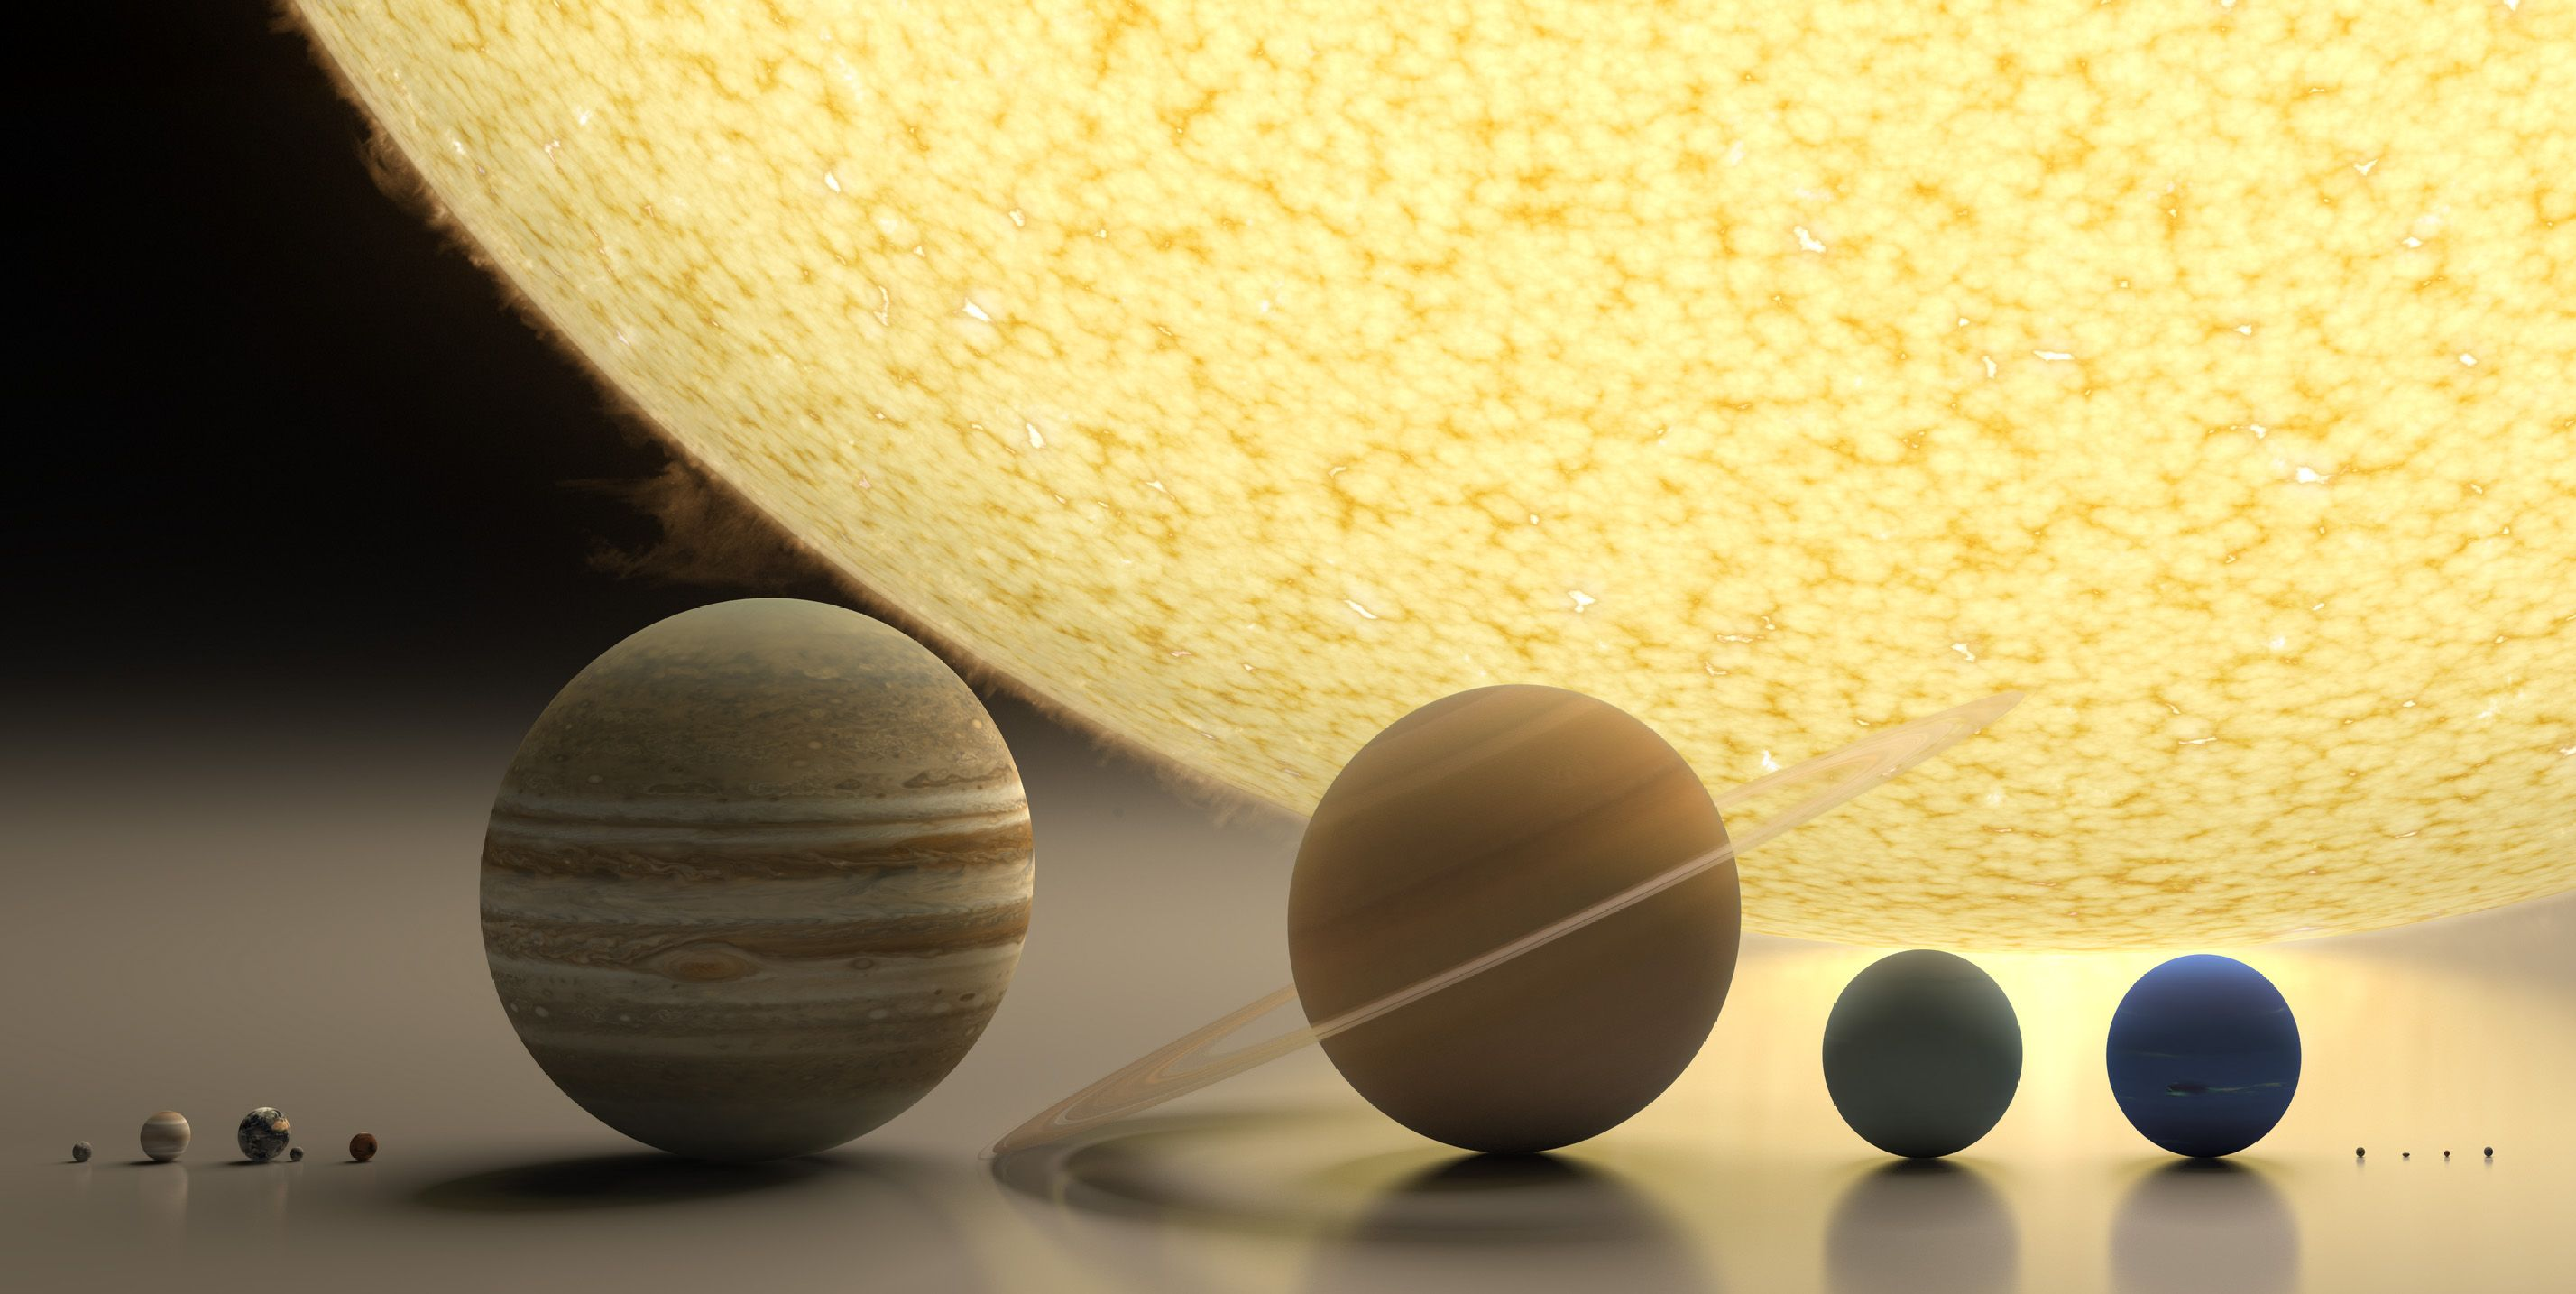
\includegraphics[width=14cm]{./figures/Astro1.pdf}
\caption{真实比例下太阳与行星的大小(来自 pinterest.com), 行星从左到右依次为水星, 金星, 地球(及月亮), 火星, 木星, 土星, 天王星, 海王星, 其他小行星} \label{Astro_fig1}
\end{figure}

恒星和行星一个显著的区别就是恒星很大, 而且会发光. 太阳是太阳系中唯一一个恒星, 其他天体都不发光, 而是反射太阳的光.

关于太阳系模型一个误区是行星的尺寸和距离, 大部分太阳系模型的比例都是完全错误的, 原因是如果按照真实比例制作模型, 要么就是行星小得看不到, 要么就是模型大得不切实际. 我们这里来构建一个符合比例的太阳系模型, 即用乒乓球来代表太阳, 再按比例计算其他长度和距离, 结果见\autoref{Astro_tab1}.

\begin{table}[ht]
\centering
\caption{太阳系的一些数据}\label{Astro_tab1}
\begin{tabular}{|c|c|c|}
\hline
 & 真实长度 & 模型长度 \\
\hline
太阳半径 & $6.96\times 10^5 \Si{km}$ & $20.0 \Si{mm}$\\
\hline
地球半径 &  $6.37\times 10^3 \Si{km}$ & $0.183 \Si{mm}$\\
\hline
地球到太阳  &  $1.46 \times 10^8 \Si{km}$ & $4.20 \Si{m}$\\
\hline
月球半径 & $1.74 \times 10^3 \Si{km}$ & $0.0500 \Si{mm}$\\
\hline
月球到地球 & $3.84 \times 10^5 \Si{km}$ &  $1.10 \Si{cm}$\\
\hline
土星半径 & $7.15 \times 10^4 \Si{km}$ & $2.05 \Si{mm}$\\
\hline
土星到太阳 & $7.79 \times 10^8 \Si{km}$ & $22.4 \Si{m}$\\
\hline
海王星到太阳 & $4.50 \times 10^9 \Si{km}$ & $129 \Si{m}$\\
\hline
最近的恒星到太阳 & $3.99 \times 10^{13} \Si{km}$ &  $1.15 \times 10^3 \Si{km}$\\
\hline
\end{tabular}
\end{table}

\subsection{星空}

\begin{figure}[ht]
\centering
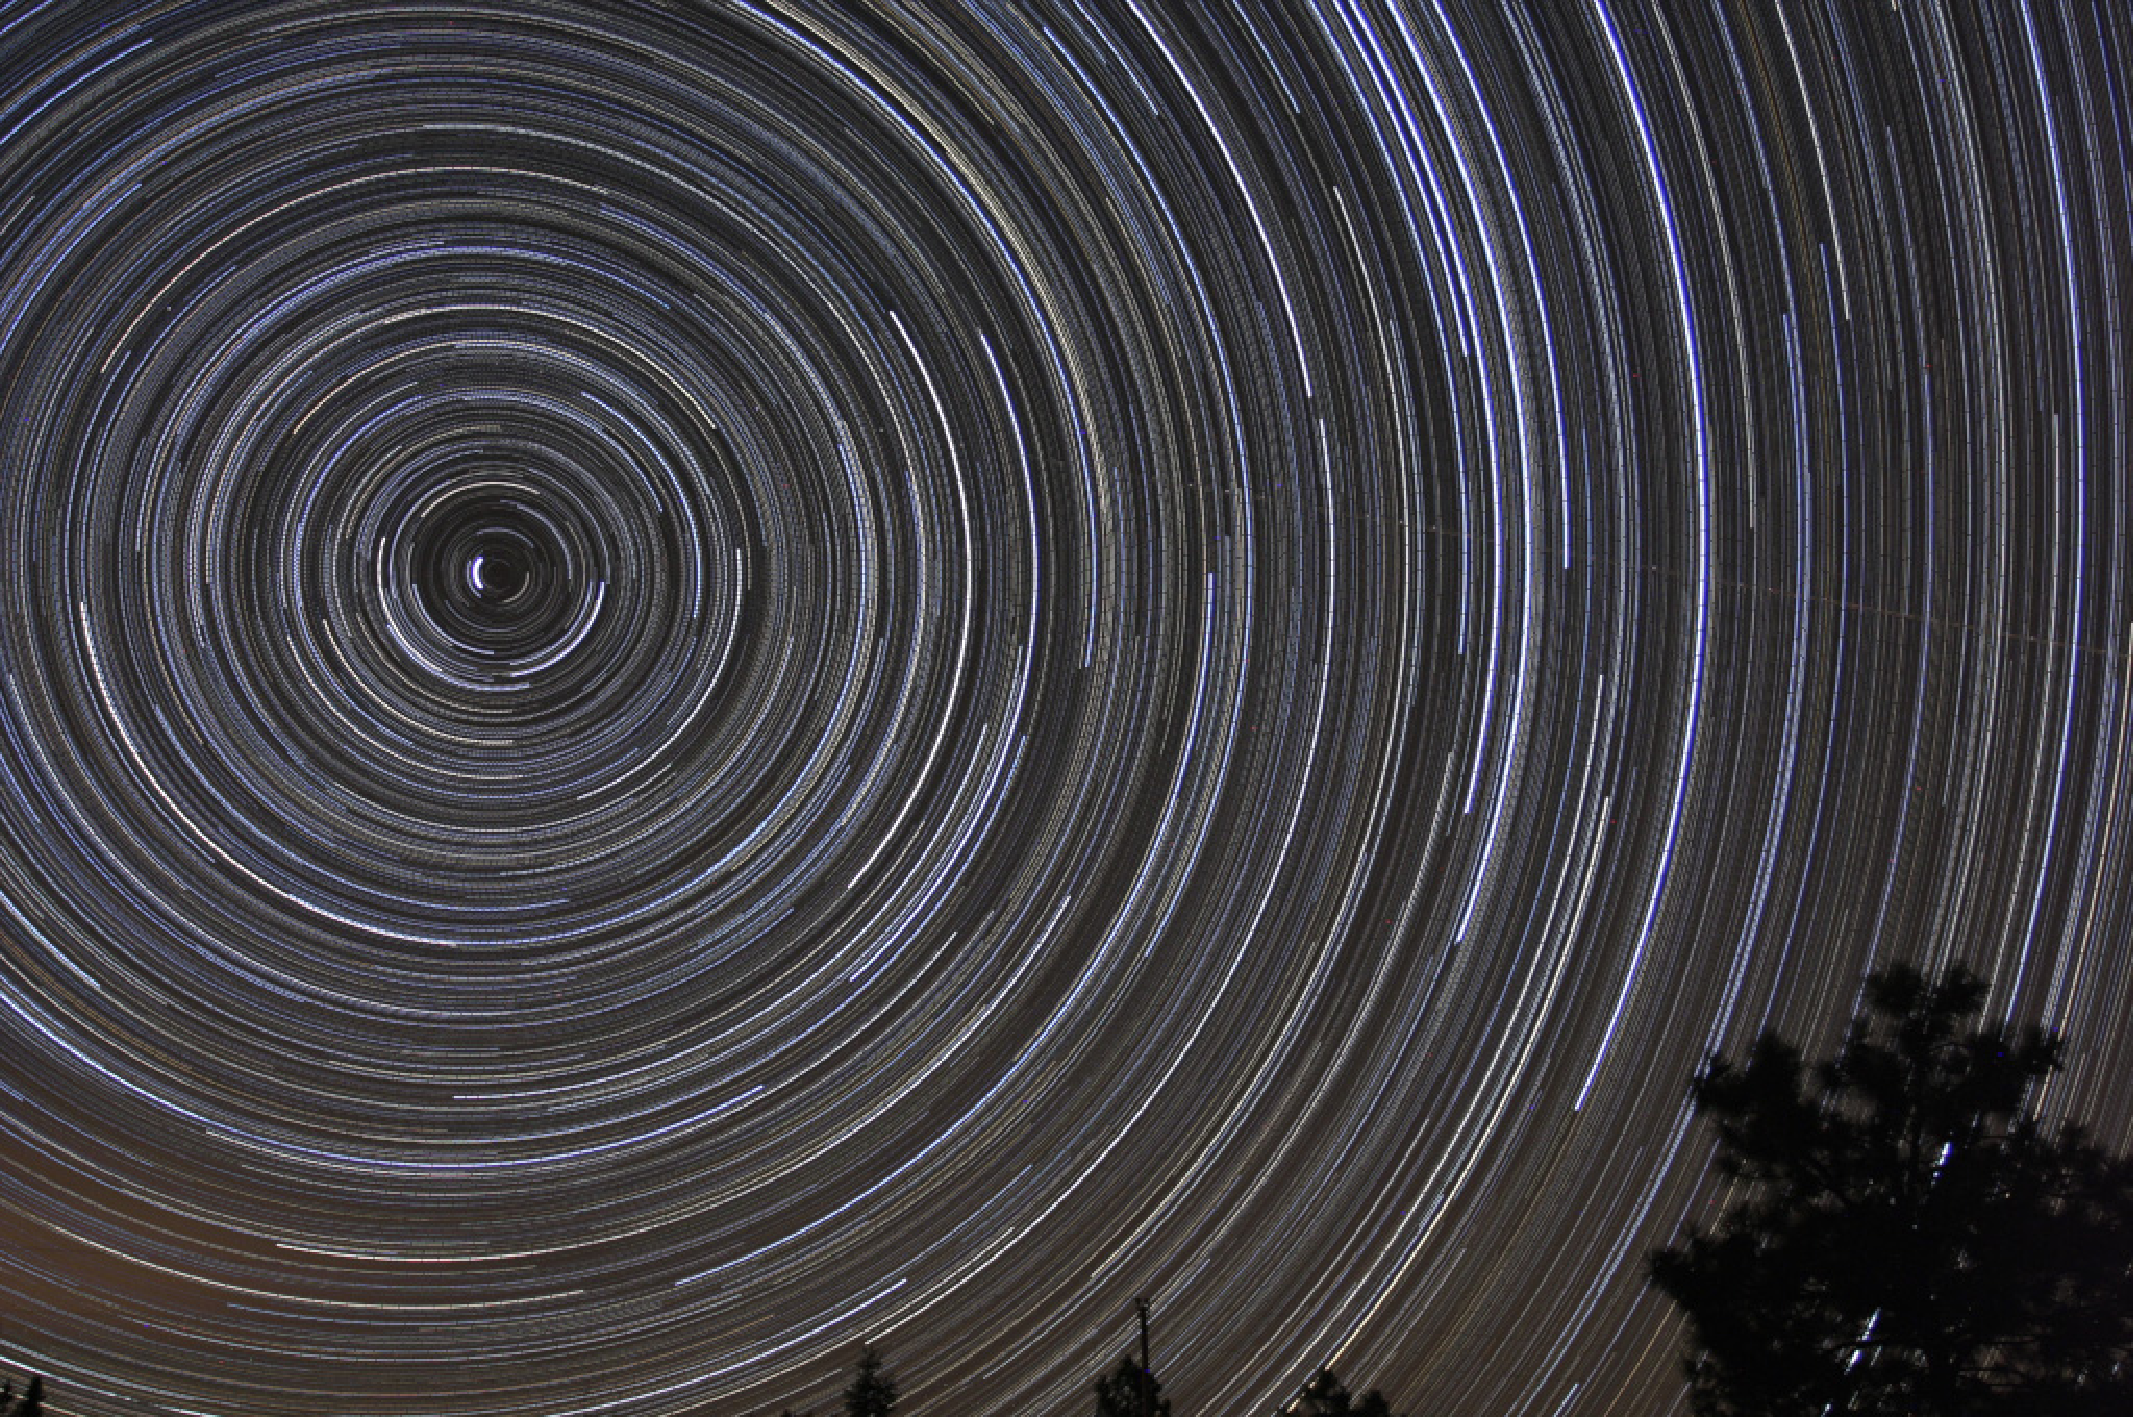
\includegraphics[width=14cm]{./figures/Astro2.pdf}
\caption{星星的轨迹(来自 burro.case.edu), 注意如果测量图中每条弧线的张角就可以计算曝光的时间} \label{Astro_fig2}
\end{figure}

除了太阳系中的天体, 肉眼或望远镜能看到的其他星星都属于恒星(注意有一些亮点是星云, 即星际尘埃而不是单个恒星), 离太阳最近的恒星叫做 Alpha Centauri (4.22 光年). 由于这些恒星的距离太远, 即使用天文望远镜也看不到它们的行星. 恒星在空中的相对位置是几乎不变的(即使太阳系以惊人的速度绕星系中心旋转, 但转一圈仍需要 2.3 亿年, 所以与其他恒星的相对位置基本保持不变).

那我们看到的星空是如何变化的呢? 由于地球每 24 小时由西向东自转一圈, 所以我们在地球上看到的星空由东向西围绕地球旋转. 长时间曝光的照片可以很好地展示星星的轨迹(\autoref{Astro_fig2}). 如果站在北极点, 那么星空的旋转中心会在正上方, 如果站在赤道, 旋转中心会在地平线上, 且南北各有一个. 如果站在南极点, 则旋转中心同样在正上方但旋转方向却与北极的相反.

一个常见的问题是为什么白天看不到星星和月亮. 这是因为白天阳光照亮了大气中的尘埃和云, 相比之下星星的亮度太暗了所以肉眼不容易看到. 许多时候月亮也会在白天出现在太阳附近, 也是因为阳光太亮不容易注意到.

下面我们来更具体地描述星空, 我们可以想象地球处于一个比地球大得多的透明球中心, 所有的星星都画在球上\footnote{显然这个模型是不真实的, 因为星星离我们的距离并不都一样, 但这对观察者来说没有影响.}, 且随透明球旋转. 我们把这个假想的球体叫做\bb{天球}. 由于天球半径远大于地球半径, 无论从地球上哪一点观察, 星星的相对分布都完全一样(如果天球只比地球大一点, 两个星星之间的视角将会随着天球的转动不断变化). 现在如果观察者站在某个纬度观测星空, 他看到的天球将如\autoref{Astro_fig3} 所示.

\begin{figure}[ht]
\centering
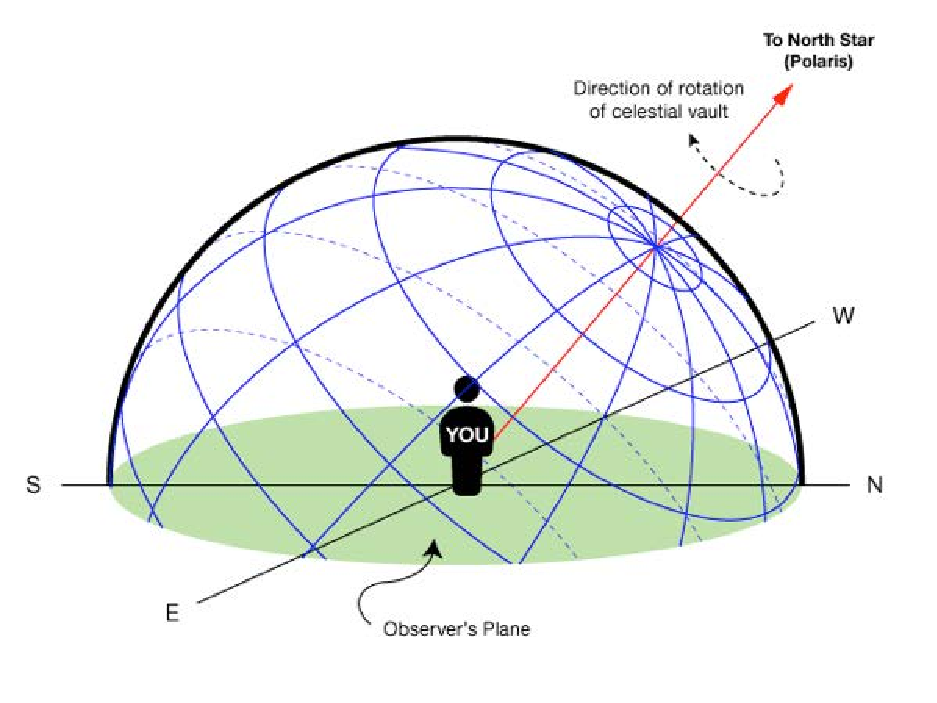
\includegraphics[width=11.5cm]{./figures/Astro3.pdf}
\caption{观星者和星空} \label{Astro_fig3}
\end{figure}

图中若观察者在北半球, 红色箭头是地轴指向北的方向, 箭头在地面投影的方向就是观察者的正北. 地轴与地面的夹角等观察者所在的纬度, 即如果观察者在北极点(北纬90°), 则地轴垂直于地面, 如果观察者在赤道(纬度为 0), 则地轴平行于地面.

在天球与红线相交的附近恰好有一颗星星, 叫做北极星. 显然, 随着天球转动, 观察者会看见北极星几乎保持静止, 而其他星星绕北极星做逆时针的圆周运动( \autoref{Astro_fig2}). 注意我们最多能看到大约一半的星空, 而另一半被地球挡住了(消失在地平线下方).

\subsection{季节与昼夜}

如(图未完成), 地球绕太阳旋转轨道所在的平面叫\bb{黄道平面}, 而地轴与黄道平面有大约 23.5° 的倾角, 所以当地球运动到太阳的一侧时, 太阳直射到北回归线(北纬 23.5° 的纬线), 这一天就叫做夏至, 当地球绕太阳旋转 90° 后, 太阳直射到赤道上, 这一天就叫做春分, 而地球再公转 90°到另一侧时, 太阳直射到南回归线, 这一天就是冬至, 再公转 90°, 阳光再次直射到赤道上, 这一天就是夏至.

回想第一节的太阳系模型, 由于地球到太阳的距离远大于二者的半径, 所以可以近似认为太阳照到地球的光都是平行的(图未完成), 这样, 任何时刻只有半个地球被照亮, 这半个地球就是白天, 而另外半个是晚上. 由于地轴的倾斜, 北半球某条纬线以上的地区在夏天会被全部被照亮, 这样无论地球自转多少, 这些地区都是白天, 这就形成了\bb{极昼}. 与此同时, 南半球某条纬线以上的地区全部没有阳光, 就形成了\bb{极夜}. 同理, 在冬天(也就是南半球的夏天)南极附近会出现极昼而北极附近出现极夜. 另外在赤道, \bb{昼长}(白天的长度)和\bb{夜长}(夜晚的长度)一年四季都相等.

% 冷暖与太阳倾角

我们重新看天球模型(仍然假设观察者在北半球), 在一天之内, 可近似认为太阳在天球的某个位置上不动, 并且随其他星星一起匀速旋转. 为了方便描述, 我们把天球也画上纬度. 冬至这天太阳会出现在天球的南纬 23.5°, 而夏至这天会出现在北纬 23.5°, 从太阳的轨迹可以看出, 夏天的昼长明显要比冬天长, 且阳光与地面更加垂直. 

不同季节的星空有什么不同.










